\section{El radar pasivo.}


El radar (radio detection  and ranging, detección y medición de distancias por onda de radio) es un sistema que usa ondas electromagnéticas para medir distancias, altitudes, direcciones y velocidades de objetos estáticos o móviles como aeronaves, barcos, vehículos motorizados, formaciones meteorológicas y el propio terreno. 
Su funcionamiento se basa en emitir un impulso de radio, que se refleja en el objetivo y se recibe típicamente en la misma posición del emisor. 
A partir de este ''eco'' se puede extraer gran cantidad de información. 
Los sistemas de radar convencionales comprenden un transmisor y un receptor, que generalmente comparten una antena común para transmitir y recibir. 
Se transmite una señal pulsada y el tiempo que tarda el pulso en viajar hasta el objeto y regresar, permite determinar la posición del objeto.

En un sistema de radar pasivo no hay un transmisor dedicado. En su lugar, el receptor utiliza transmisores de externos y mide la diferencia de tiempo de llegada entre la señal que llega directamente desde el transmisor y la señal que llega a través de la reflexión desde el objeto. 
Este esquema corresponde a un radar biestático, o sea,  es un radar donde el emisor y el receptor están separados.

\begin{figure}[h!]
\centering
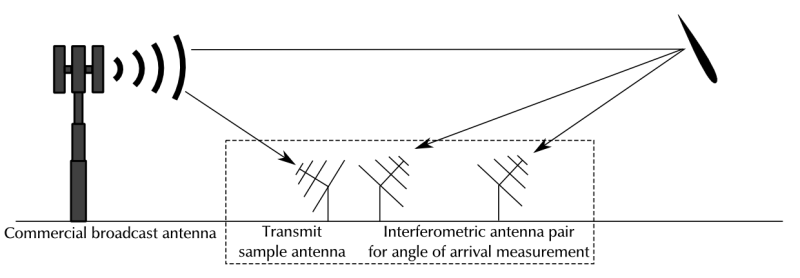
\includegraphics[width=0.8\textwidth]{fig/pasivo.png}
\caption{Frontend}
\label{fig:Radar pasivo}
\end{figure}


El movimiento del objetivo causa una tasa de cambio del rango biestático, que resulta en er shift biestático. Entonces, además del rango biestático, un radar pasivo típicamente también medirá el Doppler shift biestático del eco y también su dirección de llegada. 
Esto permite calcular la ubicación, el rumbo y la velocidad del objeto. En algunos casos, se pueden emplear múltiples transmisores y/o receptores para realizar varias mediciones independientes del rango biestático, Doppler y rodamiento y, por lo tanto, mejorar significativamente la precisión final.


La descripción anterior asume que la forma de onda del transmisor que se está explotando posee una función de ambigüedad del radar utilizable y, por lo tanto, la correlación cruzada produce un resultado útil. Algunas señales de transmisión, como la televisión analógica, contienen una estructura en el dominio del tiempo que produce un resultado altamente ambiguo o inexacto cuando se realiza una correlación cruzada. En este caso, el procesamiento descrito anteriormente es ineficaz. Sin embargo, si la señal contiene un componente onda continua (CW), como un tono de portadora, es posible detectar y rastrear objetivos de una forma alternativa. Con el tiempo, los objetivos en movimiento impondrán un cambio Doppler cambiante y la dirección de llegada en el tono de CW que es característico de la ubicación, la velocidad y el rumbo del objetivo. 
Se han desarrollado sistemas de radar pasivo que emplean señales Televisión analógica, radio FM señales y estaciones de teléfono celular. Pero, las señales satelitales son inadecuadas para el uso de radar pasivo, ya sea porque las potencias son demasiado bajas o porque las órbitas de los satélites son tales que la iluminación es demasiado infrecuente. 


\subsection{Principio de funcionamiento}. 

En un sistema de radar convencional, el tiempo de transmisión del pulso y la forma de onda transmitida son exactamente conocidos. Esto permite que el rango del objeto se calcule fácilmente y que se use un filtro adaptativo para lograr una relación señal/ruido óptima en el receptor. 
Un filtro adaptado (''matched filter'') es un sistema lineal invariante cuya función principal es detectar la presencia de una señal conocida, o referencia, dentro de una señal recibida. La señal a la salida del filtro será la correlación de la señal referencia con la señal desconocida. Este procedimiento es equivalente a realizar la convolución de la señal desconocida con una versión retardada de la señal, que usamos como referencia.
Un radar pasivo no tiene esta información directamente y, por lo tanto, debe usar un canal receptor dedicado (conocido como "canal de referencia") para monitorear cada transmisor.

Un radar pasivo emplea típicamente los siguientes pasos de procesamiento:
\begin{itemize}
    \item Recepción de la señal directa desde el transmisor y desde la región de vigilancia en receptores digitales, lineales y de bajo nivel de ruido dedicados
    \item Conformación de la traza para determinar la dirección de llegada de las señales y el rechazo espacial de una fuerte interferencia en banda.
    \item Filtro adaptado para cancelar cualquier retorno de señal directo no deseado en el canal de vigilancia.
    \item Condicionamiento de señal específico del transmisor.
    \item Correlación cruzada del canal de referencia con los canales de referencia para determinar el rango bi-estático del objeto y el Doppler.
    \item Asociación y fusión de las líneas de cada transmisor para formar la estimación final de la ubicación, el rumbo y la velocidad de un objeto.
\end{itemize}


Estos se describen con mayor detalle en las secciones a continuación.


\subsubsection{Sistema receptor}
Un sistema de radar pasivo debe detectar reflexiones de la señal producidas por los objetivos muy pequeños en presencia de interferencias muy fuertes y continuas. Esto contrasta con un radar convencional, que escucha ecos durante los períodos de silencio entre cada transmisión de pulso. Como resultado, es esencial que el receptor tenga una baja cifra de ruido, alta rango dinámico y alta linealidad. A pesar de esto, los ecos recibidos están normalmente muy por debajo del piso de ruido y el sistema tiende a estar limitado por el ruido externo (debido a la recepción de la propia señal transmitida, más la recepción de otros transmisores en banda distantes). 

\subsubsection{Condicionamiento de señal}
Con algunos tipos de transmisores, es necesario realizar algún acondicionamiento específico de la señal para el transmisor antes del procesamiento de correlación cruzada. Esto puede incluir el filtrado de paso de banda analógico de alta calidad de la señal, la ecualización del canal para mejorar la calidad de la señal de referencia, la eliminación de estructuras no deseadas en las señales digitales para mejorar la función de ambigüedad del radar o incluso la reconstrucción completa de la señal de referencia del Señal digital recibida.

\subsubsection{Filtrado adaptativo}
La principal limitación en el rango de detección para la mayoría de los sistemas de radar pasivos es la relación señal-interferencia, debido a la señal directa grande y constante recibida del transmisor. Para eliminar esto, se puede usar un filtro adaptativo para eliminar la señal directa en un proceso similar al control de ruido activo. Este paso es esencial para garantizar que los lóbulos laterales de rango / Doppler de la señal directa no enmascaren los ecos más pequeños en la siguiente etapa de correlación cruzada.

\subsubsection{Procesamiento de correlación cruzada}
El paso de procesamiento de la clave en un radar pasivo es correlación cruzada. Este paso actúa como filtro coincidente y también proporciona las estimaciones del rango biestático y el desplazamiento Doppler biestático de cada eco objetivo. La mayoría de las señales de transmisión analógicas y digitales son de naturaleza similar al ruido, y como consecuencia, tienden a correlacionarse solo con ellas mismas. Esto presenta un problema con los objetivos en movimiento, ya que el Doppler shift impuesto en el eco significa que no se correlacionará con la señal directa del transmisor. Como resultado, el procesamiento de correlación cruzada debe implementar un banco de filtros coincidentes, cada uno combinado con un cambio Doppler objetivo diferente. Usualmente se usan implementaciones eficientes del procesamiento de correlación cruzada basado en la transformada de Fourier discreta.

\subsubsection{Detección de blancos}
Los objetivos se detectan en la superficie de correlación cruzada aplicando un umbral adaptativo y declarando que todos los rendimientos por encima de esta superficie son objetivos. Por lo general, se utiliza un algoritmo estándar de promedio de celda tasa constante de falsas alarma (CFAR, del acrónimo inglés Constant False Alarm Rate).

En una configuración biestática simple (un transmisor y un receptor) es posible determinar la ubicación del objetivo simplemente calculando el punto de intersección del rodamiento con el rango biestático elipse. Sin embargo, los errores en el rumbo y el alcance tienden a hacer que este enfoque sea bastante inexacto. Un mejor enfoque es estimar el estado objetivo (ubicación, rumbo y velocidad) a partir del conjunto completo de medición del rango bi-estático, el rumbo y el Doppler utilizando un filtro no lineal, como el filtro de Kalman.



